\documentclass[11pt, letterpaper, notitlepage]{article}

\usepackage{multicol}
\usepackage{fancyhdr}
\usepackage[margin=0.75in]{geometry}
\usepackage{graphicx}
\PassOptionsToPackage{hyphens}{url}\usepackage{hyperref}
\usepackage{authblk}
\usepackage{amsmath, amssymb}
\usepackage[hypcap=false]{caption}
\usepackage{float}
\graphicspath{ {./images/}}

\usepackage{biblatex}
\addbibresource{PNNL-CT.bib}

%-------------Custom Abstract Def----------------
% Modified abstract command in order to better suit the styles common in other papers in the field.
\def\abstract{\if@twocolumn
\section*{Abstract}
\else
% modified quotation macro from latex.tex
\list{}{\listparindent 1.5em \topsep 1pt \parskip 0pt \partopsep 0pt
 \itemindent\listparindent
        \setlength\rightmargin{5em}
        \setlength\leftmargin{5em}
 \parsep 0pt plus 1pt}\item[]
% end of modified quotation macro
\noindent \footnotesize{\bf Abstract.}
 \ignorespaces %  -SLK-00Mar12> 
\fi}
\def\endabstract{\if@twocolumn\else\endlist\fi\bigskip\smallskip}

%-------------Title Details----------------------
\title{%
  An Exploration of Image Stitching as a Linear Optimization Problem\\
  \large \vspace{1em}\textbf{Initial Project Proposal}
}

%\author[1]{Thomas Pasfield}

\author{Thomas Pasfield}
\author{Madeline Gorman}


\affil{Embry-Riddle Aeronautical University, Daytona Beach, FL.}

%-------------Header/Footer Modification---------
\pagestyle{fancy}
\fancyhead{}
\fancyhead[L]{Image Stitching via Linear Optimization}
\fancyhead[R]{\thepage}
\fancyfoot{}
\setlength{\headheight}{13.59999pt}
\addtolength{\topmargin}{-1.59999pt}


\newenvironment{Figure}
  {\par\medskip\noindent\minipage{\linewidth}}
  {\endminipage\par\medskip}

\begin{document}
\maketitle

%\begin{abstract}
%\end{abstract}

\begin{multicols}{2}
\section{Introduction}
Image stitching provides a useful tool for both consumers and for industry. In consumer products, people generally encounter it in the form of panoramic images on their phones. In industry, it finds applications in anything from photogrammetry to remote sensing. While it isn't a particularly new technology, it still has broad application and has a simple entry-point. We feel that this makes it ideal as a student project.

In computational imaging, the most common representation of imaging is in the form of a linear system. In applications such as deblurring, edge detection, and other filtering, it is common to see a formulation such as Equation \ref{eqn:range-form}.

\begin{equation}
  \label{eqn:range-form}
  \vec{\mathbf{b}} = A\vec{\mathbf{x}} + \vec{\varepsilon}
\end{equation}

In this form, $\vec{\mathbf{x}}$ and $\vec{\mathbf{b}}$ represent $mn\times 1$ sized vectors, equivalent to stacking the columns of the image atop each other sequentially. $A$ represents the transformation matrix, which acts upon the range of the image. This must be of size $mn\times mn$. $\vec{\varepsilon}$ often represents the residual, or random noise. It is not adequate to represent an image as a linear transformation upon its range in this problem, as we need to warp and translate the images rather than filter them.

To better address this problem, we will approach the image processing in the domain of the image instead. We want to modify the coordinate space rather than the values at those coordinates. This new formulation is shown in Equation \ref{eqn:domain-form}.

\begin{equation}
  \label{eqn:domain-form}
  \vec{\mathbf{b}} = T\vec{\mathbf{x}}
\end{equation}

Unlike the form in Equation \ref{eqn:range-form}, $\vec{\mathbf{x}}$ and $\vec{\mathbf{b}}$ represent $2\times1$ vectors of the coordinate, and the transformation matrix is simply represented by $T$, which is $2\times2$. This method is performed on each pixel individually, which allows for efficient parallelization. All the image warping and transformations which we must perform can be represented by this form with ease.

As we approach this problem, we expect to encounter transformations such as:
\begin{itemize}
  \item Translation
  \item Rotation
  \item Scaling/Aspect
  \item Affine Transformation
  \item Perspective Transformation
  \item Barrel Distortion
\end{itemize}

\section{Planned Approach and Implementation}

We plan to approach this problem via optimization, where the results are scored by some metric, and we iterate to minimize this score. Metrics based on the overlap of pixels will certainly be computationally inefficient but will be quite simple to set up. This may make a good first iteration for our work, and we can expand upon this and implement a feature-detection based approach, with algorithms such as SIFT.

Our primary focus is on the optimization algorithms rather than the computational efficiency of other components. This problem will require multi-variable optimization, of which we don't yet know the difficulty of. At the very least we have parameters such as the x and y components for translation and scaling, an angle $\theta$ for rotation. Parameters for the affine and perspective transformations will be fairly similar, to the extent that affine may likely be replaced by perspective if we encounter too many variables. We expect a minimum of 4 additional parameters for each of these transforms that we must tune.

Our work will be performed using Python and managed via a GitHub repository. We will make extensive use of the Numpy and Scipy libraries. We will likely use \verb|scipy.optimize| in our early implementation to ensure that our model functions as expected before we implement our own optimization. We may perform early image operations via the Python Image Library (PIL) or OpenCV if necessary.

If we reach our stretch goals related to blending the images, OpenCV will likely be utilized to perform these range transformations, as they are purely for our qualitative review, and are not a primary focus of this work.

\section{Project Goals}
The focus of this work is to implement an optimization-driven image stitching approach. It does not seek to develop any new methods.

\subsection*{Primary Goal}
We seek to be capable of stitching at least 3 grayscale images, each of a size of $100\times100$ pixels or greater, with a very rough initial guess provided by the user. We will operate within at least a rectilinear coordinate space, and we seek to apply at least 3 types of optimization.

\subsection*{Stretch Goals}
Provided that we complete our primary goal, we would like to pursue some additional features and capabilities. Many of these are qualitative in nature.

\begin{enumerate}
  \item Add support for color images.\\
        We expect this to be fairly simple, but to triple the computations performed.
  \item Add support for range transformations.\\
        Modifying exposure, contrast, white balance, and other range-based transformative properties, we can create a more visually appealing output.
  \item Add support for more coordinate spaces.\\
        This allows for a much more accurate output, but is much more difficult for us to intuitively approach.
\end{enumerate}



\section{Data Availability and Sources}

Computational imaging is a broad enough field that they have well-established standard test images and datasets. There are many resources out there which we can utilize to test out methods on, such as:

\begin{itemize}
  \item \url{https://github.com/visionxiang/Image-Stitching-Dataset}
  \item \url{https://paperswithcode.com/dataset/udis-d}
  \item \url{https://paperswithcode.com/datasets?task=image-stitching&mod=images}
\end{itemize}

We could also utilize other public datasets such as archived images from NASA's Mars2020 Perseverance Rover. An example of an image stitch of this data can be seen in Figure \ref{fig:rover}.

\begin{Figure}
  \centering  
  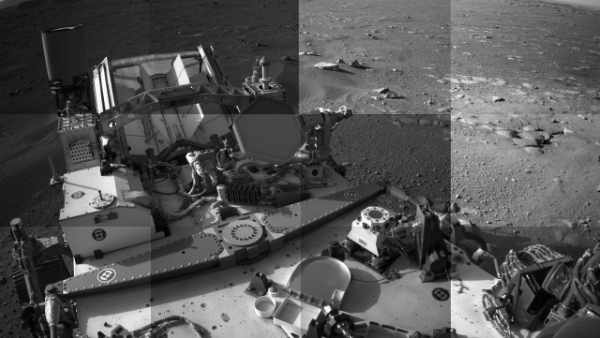
\includegraphics[width=3in]{images/stitch.png}
  \captionof{figure}{\emph{A manually stitched image series of the Mars2020 Perseverance Rover. This is performed within rectilinear space with translation and scale operations. No range transformation was performed. This was performed by Thomas.}}
  \label{fig:rover}
\end{Figure}

It is also possible for us to use free open-source software such as Blender to generate our own ideal image data. This could allow us to create ideal data without distortion, camera shake, or other inconveniences. This process would be very simple and could be done within 2-3 days easily.

%\printbibliography

\end{multicols}

\end{document}

% PLACEHOLDERS FOR FUTURE FIGURES
%\begin{Figure}
%  \centering
%  \includegraphics[width=3in]{esf}
%  \captionof{figure}{A demonstration of the process of determining an ESF from an image. Notice the width of the blur in the image and how it relates to the edge spread shown in the ESF plot. Note that these are optimal examples without any noise present.}
%  \label{fig:ESF}
%\end{Figure}


%\vspace{1em}
%\begin{Figure}
%  \centering
%  \begin{tabular}{r|r|r|r|r|r|r}
%         & 128$^2$ & 256$^2$ & 512$^2$ & 1024$^2$ & 2048$^2$ & 4000$^2$ \\ \hline \hline
%      Half & 0.5 GB & 8.6 GB & 137.4 GB & 2199.0 GB & 35184.4 GB & 512000.0 GB \\
%      Single & 1.1 GB & 17.2 GB & 274.9 GB & 4398.0 GB & 70368.7 GB & 1024000.0 GB \\
%      Double & 2.1 GB & 34.4 GB & 549.8 GB & 8796.1 GB & 140737.5 GB & 2048000.0 GB
%  \end{tabular}
%  \captionof{table}{A table showing the size requirements for storing matrices of various sizes and precision in memory. Its exponential growth presents a significant problem for execution. The final column represents the size of image that the Cygnus x-ray machine takes. The memory capacity needed to utilize the linear model on the full data greatly exceeds any machines that we have access to, and even that of many of the world's supercomputers.}
%  \label{tab:size}
%\end{Figure}